%%%%%%%%%%%%%%%%%%%%%%%%%%%%%%%%%%%%%%%%%%%%%%%%%%%%%%%%%%%%
% 3.4 AFFINE GEOMETRY
% The Composition of Advanced Mathematics
%%%%%%%%%%%%%%%%%%%%%%%%%%%%%%%%%%%%%%%%%%%%%%%%%%%%%%%%%%%%

\section{Affine Geometry}
\label{sec:affine-geometry}

\prerequisite{
Euclidean Geometry from \cref{sec:euclidean-geometry},
Analytic / Coordinate Geometry from
\cref{sec:analytic-coordinate-geometry},
Vector Geometry from \cref{sec:vector-geometry},
and Linear Algebra from \cref{sec:linear-algebra}.
}

\learningobjectives{
By the end of this section, the reader should be able to:
\begin{itemize}
    \item distinguish affine geometry from Euclidean and vector geometry;
    \item explain the difference between points and vectors in an affine space;
    \item describe affine lines, planes, and higher-dimensional affine subspaces;
    \item form and interpret affine combinations;
    \item recognize barycentric and convex combinations;
    \item characterize affine independence;
    \item compute affine hulls and understand affine dimension;
    \item use barycentric coordinates for points in simplices;
    \item identify affine transformations and their matrix form;
    \item determine which geometric properties are preserved by affine transformations;
    \item understand translations as affine rather than linear transformations;
    \item use homogeneous coordinates to represent affine transformations;
    \item recognize parallelism and ratios as fundamental affine invariants;
    \item connect affine geometry with convex geometry, projective geometry,
    computational geometry, and computer graphics.
\end{itemize}
}

%%%%%%%%%%%%%%%%%%%%%%%%%%%%%%%%%%%%%%%%%%%%%%%%%%%%%%%%%%%%
\subsection{What Is Affine Geometry?}
\label{subsec:what-is-affine-geometry}
%%%%%%%%%%%%%%%%%%%%%%%%%%%%%%%%%%%%%%%%%%%%%%%%%%%%%%%%%%%%

Euclidean geometry studies properties involving lengths, angles, circles,
perpendicularity, and distance.

Affine geometry keeps some geometric structure while discarding others.

\begin{definitionbox}{Affine Geometry}
\emph{Affine geometry} studies geometric properties preserved by affine
transformations.

These include incidence, collinearity, parallelism, ratios along parallel
directions, affine combinations, and affine dimension.
\end{definitionbox}

Affine geometry does \emph{not} generally preserve:

\begin{itemize}
    \item lengths;
    \item angles;
    \item perpendicularity;
    \item circles;
    \item ordinary areas or volumes.
\end{itemize}

Thus affine geometry lies conceptually between linear algebra and projective
geometry.

%%%%%%%%%%%%%%%%%%%%%%%%%%%%%%%%%%%%%%%%%%%%%%%%%%%%%%%%%%%%
\subsection{Euclidean Versus Affine Geometry}
\label{subsec:euclidean-versus-affine}
%%%%%%%%%%%%%%%%%%%%%%%%%%%%%%%%%%%%%%%%%%%%%%%%%%%%%%%%%%%%

Consider a square.

Under an affine transformation, it may become a parallelogram.

\begin{centereddiagram}
\begin{tikzpicture}[scale=0.75]
\draw[thick] (0,0)--(2,0)--(2,2)--(0,2)--cycle;
\node at (1,-0.5) {square};

\draw[-{Latex[length=3mm]},thick] (2.8,1)--(4.2,1);
\node[above] at (3.5,1) {affine map};

\draw[thick] (5,0)--(7.5,0)--(8.5,2)--(6,2)--cycle;
\node at (6.75,-0.5) {parallelogram};
\end{tikzpicture}
\end{centereddiagram}

The transformation may change:

\[
\text{lengths},\qquad
\text{angles},\qquad
\text{area}.
\]

But it preserves:

\[
\text{lines},\qquad
\text{parallelism},\qquad
\text{collinearity}.
\]

The square and parallelogram are therefore equivalent from the affine
viewpoint.

%%%%%%%%%%%%%%%%%%%%%%%%%%%%%%%%%%%%%%%%%%%%%%%%%%%%%%%%%%%%
\subsection{Points and Vectors}
\label{subsec:affine-points-vectors}
%%%%%%%%%%%%%%%%%%%%%%%%%%%%%%%%%%%%%%%%%%%%%%%%%%%%%%%%%%%%

One of the most important distinctions in affine geometry is the distinction
between \emph{points} and \emph{vectors}.

A vector describes a displacement.

A point describes a location.

If \(P\) and \(Q\) are points, then

\[ Q-P \]

is interpreted as the vector from \(P\) to \(Q\).

However, adding two points such as

\[ P+Q \]

has no intrinsic affine meaning.

By contrast, adding a vector to a point does make sense:

\[ P+\mathbf{v}. \]

The result is another point.

\begin{importantbox}
An affine space has points and displacement vectors, but it has no preferred
origin.

Choosing an origin allows the affine space to be represented using a vector
space, but the choice of origin is additional structure.
\end{importantbox}

%%%%%%%%%%%%%%%%%%%%%%%%%%%%%%%%%%%%%%%%%%%%%%%%%%%%%%%%%%%%
\subsection{Affine Space}
\label{subsec:affine-space}
%%%%%%%%%%%%%%%%%%%%%%%%%%%%%%%%%%%%%%%%%%%%%%%%%%%%%%%%%%%%

\begin{definitionbox}{Affine Space}
An \emph{affine space} consists of a set of points together with a vector
space of translations acting freely and transitively on those points.
\end{definitionbox}

Informally, this means:

\begin{itemize}
    \item vectors can move points;
    \item any point can be moved to any other point by exactly one vector;
    \item no point is inherently distinguished as the origin.
\end{itemize}

If the underlying vector space is \(V\), the affine space is often denoted

\[ A. \]

For points \(P,Q\in A\),

\[ Q-P\in V. \]

For \(P\in A\) and \(\mathbf{v}\in V\),

\[ P+\mathbf{v}\in A. \]

%%%%%%%%%%%%%%%%%%%%%%%%%%%%%%%%%%%%%%%%%%%%%%%%%%%%%%%%%%%%
\subsection{Affine Space as a Translated Vector Space}
\label{subsec:translated-vector-space}
%%%%%%%%%%%%%%%%%%%%%%%%%%%%%%%%%%%%%%%%%%%%%%%%%%%%%%%%%%%%

Once a point \(O\) is chosen as an origin, every point \(P\) can be associated
with the vector

\[ P-O. \]

This produces coordinates.

However, another choice of origin gives different coordinate vectors.

The underlying affine relationships remain unchanged.

\begin{centereddiagram}
\begin{tikzpicture}[scale=0.9]
\fill (0,0) circle (2pt);
\fill (4,2) circle (2pt);
\fill (1,3) circle (2pt);

\node[below] at (0,0) {\(O\)};
\node[right] at (4,2) {\(P\)};
\node[left] at (1,3) {\(O'\)};

\draw[-{Latex[length=3mm]},thick] (0,0)--(4,2);
\draw[-{Latex[length=3mm]},thick] (1,3)--(4,2);

\node[below right] at (2,1) {\(P-O\)};
\node[above right] at (2.4,2.6) {\(P-O'\)};
\end{tikzpicture}
\end{centereddiagram}

The coordinates change, but the point \(P\) itself does not.

%%%%%%%%%%%%%%%%%%%%%%%%%%%%%%%%%%%%%%%%%%%%%%%%%%%%%%%%%%%%
\subsection{Affine Combinations}
\label{subsec:affine-combinations}
%%%%%%%%%%%%%%%%%%%%%%%%%%%%%%%%%%%%%%%%%%%%%%%%%%%%%%%%%%%%

Vector Geometry introduced weighted combinations whose coefficients sum to
one.

These combinations are fundamental in affine geometry.

\begin{definitionbox}{Affine Combination}
Given points \(P_1,\ldots,P_k\), an \emph{affine combination} is an
expression

\[
\boxed{
\lambda_1P_1+\cdots+\lambda_kP_k
}
\]

where

\[
\boxed{
\lambda_1+\cdots+\lambda_k=1.
}
\]
\end{definitionbox}

The lowercase Greek letter \(\lambda\) is \emph{lambda}, pronounced
``LAM-duh.''

The condition that the coefficients sum to \(1\) makes the expression
independent of the choice of origin.

%%%%%%%%%%%%%%%%%%%%%%%%%%%%%%%%%%%%%%%%%%%%%%%%%%%%%%%%%%%%
\subsection{Why Must the Coefficients Sum to One?}
\label{subsec:affine-coefficients-sum-one}
%%%%%%%%%%%%%%%%%%%%%%%%%%%%%%%%%%%%%%%%%%%%%%%%%%%%%%%%%%%%

Suppose coordinates are measured relative to an origin \(O\).

If the origin is shifted by a vector \(\mathbf{a}\), then each point
coordinate changes by the same amount:

\[ P_i\mapsto P_i+\mathbf{a}. \]

An affine combination becomes

\[
\sum_{i=1}^{k}\lambda_i(P_i+\mathbf{a})
=
\sum_{i=1}^{k}\lambda_iP_i
+
\left(\sum_{i=1}^{k}\lambda_i\right)\mathbf{a}.
\]

If

\[ \sum_{i=1}^{k}\lambda_i=1, \]

then

\[
\sum_{i=1}^{k}\lambda_i(P_i+\mathbf{a})
=
\left(\sum_{i=1}^{k}\lambda_iP_i\right)+\mathbf{a}.
\]

Thus the resulting point transforms exactly as a point should under a change
of origin.

This explains why the coefficient condition is intrinsic to affine
geometry.

%%%%%%%%%%%%%%%%%%%%%%%%%%%%%%%%%%%%%%%%%%%%%%%%%%%%%%%%%%%%
\subsection{The Affine Line Through Two Points}
\label{subsec:affine-line-two-points}
%%%%%%%%%%%%%%%%%%%%%%%%%%%%%%%%%%%%%%%%%%%%%%%%%%%%%%%%%%%%

Let \(P\neq Q\).

The line through \(P\) and \(Q\) can be written

\[ \boxed{L=\{(1-t)P+tQ:t\in\R\}.} \]

Because

\[ (1-t)+t=1, \]

every point on the line is an affine combination of \(P\) and \(Q\).

Equivalently,

\[ \boxed{L=\{P+t(Q-P):t\in\R\}.} \]

The second form emphasizes a base point and a direction vector.

%%%%%%%%%%%%%%%%%%%%%%%%%%%%%%%%%%%%%%%%%%%%%%%%%%%%%%%%%%%%
\subsection{Segments and Rays}
\label{subsec:affine-segments-rays}
%%%%%%%%%%%%%%%%%%%%%%%%%%%%%%%%%%%%%%%%%%%%%%%%%%%%%%%%%%%%

The parameter range determines which part of the affine line is obtained.

For

\[ P+t(Q-P), \]

we have:

\[
\begin{array}{c|c}
\textbf{Parameter} & \textbf{Geometric Set}\\
\hline
t\in\R & \text{entire line}\\
0\leq t\leq1 & \text{segment from \(P\) to \(Q\)}\\
t\geq0 & \text{ray from \(P\) through \(Q\)}
\end{array}
\]

The segment is therefore the set of convex combinations of two points.

%%%%%%%%%%%%%%%%%%%%%%%%%%%%%%%%%%%%%%%%%%%%%%%%%%%%%%%%%%%%
\subsection{Midpoints}
\label{subsec:affine-midpoints}
%%%%%%%%%%%%%%%%%%%%%%%%%%%%%%%%%%%%%%%%%%%%%%%%%%%%%%%%%%%%

The midpoint of \(P\) and \(Q\) is

\[
\boxed{
M=\frac12P+\frac12Q.
}
\]

Since

\[ \frac12+\frac12=1, \]

the midpoint is an affine combination.

Affine transformations preserve midpoints.

This fact does not require preservation of distance.

%%%%%%%%%%%%%%%%%%%%%%%%%%%%%%%%%%%%%%%%%%%%%%%%%%%%%%%%%%%%
\subsection{Worked Example: Affine Combination}
\label{subsec:worked-affine-combination}
%%%%%%%%%%%%%%%%%%%%%%%%%%%%%%%%%%%%%%%%%%%%%%%%%%%%%%%%%%%%

\begin{workedexamplebox}{Computing an Affine Combination}

Let

\[ P=(1,2),\qquad Q=(5,6). \]

Find the point

\[ R=\frac14P+\frac34Q. \]

\begin{tabularx}{\textwidth}{@{}>{\raggedright\arraybackslash}p{0.43\textwidth}X@{}}
Verify the coefficients sum to one. &
\(\frac14+\frac34=1\)\\
Substitute the coordinates. &
\(R=\frac14(1,2)+\frac34(5,6)\)\\
Combine coordinates. &
\(R=\left(\frac14+\frac{15}{4},\frac12+\frac{18}{4}\right)\)\\
Simplify. &
\(R=(4,5)\)
\end{tabularx}

\begin{answerbox}
\[ \boxed{R=(4,5)} \]
\end{answerbox}
\end{workedexamplebox}

%%%%%%%%%%%%%%%%%%%%%%%%%%%%%%%%%%%%%%%%%%%%%%%%%%%%%%%%%%%%
\subsection{Affine Subspaces}
\label{subsec:affine-subspaces}
%%%%%%%%%%%%%%%%%%%%%%%%%%%%%%%%%%%%%%%%%%%%%%%%%%%%%%%%%%%%

Linear subspaces must contain the zero vector.

Affine subspaces need not contain the origin.

\begin{definitionbox}{Affine Subspace}
An \emph{affine subspace} of a vector space \(V\) is a translated linear
subspace of the form

\[ \boxed{P+W=\{P+\mathbf{w}:\mathbf{w}\in W\},} \]

where \(P\) is a point and \(W\) is a linear subspace.
\end{definitionbox}

The linear subspace \(W\) describes the directions available within the
affine subspace.

%%%%%%%%%%%%%%%%%%%%%%%%%%%%%%%%%%%%%%%%%%%%%%%%%%%%%%%%%%%%
\subsection{Linear Versus Affine Subspaces}
\label{subsec:linear-versus-affine-subspaces}
%%%%%%%%%%%%%%%%%%%%%%%%%%%%%%%%%%%%%%%%%%%%%%%%%%%%%%%%%%%%

Consider the lines

\[ y=2x \]

and

\[ y=2x+3. \]

The first passes through the origin and corresponds to a one-dimensional
linear subspace of \(\R^2\).

The second is parallel to the first but does not pass through the origin.

It is an affine subspace, but not a linear subspace.

\begin{centereddiagram}
\begin{tikzpicture}[scale=0.65]
\draw[->] (-3,0)--(4,0) node[right] {\(x\)};
\draw[->] (0,-3)--(0,5) node[above] {\(y\)};

\draw[thick,domain=-1.5:2] plot (\x,{2*\x});
\draw[thick,dashed,domain=-3:0.8] plot (\x,{2*\x+3});

\node[right] at (1.7,3.4) {\(y=2x\)};
\node[left] at (-1,1) {\(y=2x+3\)};
\end{tikzpicture}
\end{centereddiagram}

%%%%%%%%%%%%%%%%%%%%%%%%%%%%%%%%%%%%%%%%%%%%%%%%%%%%%%%%%%%%
\subsection{Direction Space}
\label{subsec:affine-direction-space}
%%%%%%%%%%%%%%%%%%%%%%%%%%%%%%%%%%%%%%%%%%%%%%%%%%%%%%%%%%%%

If an affine subspace is written

\[ A=P+W, \]

then \(W\) is called its \emph{direction space}.

Different choices of base point produce the same affine subspace.

If \(Q\in A\), then

\[ A=Q+W. \]

Thus the base point is not unique, but the direction space is.

%%%%%%%%%%%%%%%%%%%%%%%%%%%%%%%%%%%%%%%%%%%%%%%%%%%%%%%%%%%%
\subsection{Affine Planes}
\label{subsec:affine-planes}
%%%%%%%%%%%%%%%%%%%%%%%%%%%%%%%%%%%%%%%%%%%%%%%%%%%%%%%%%%%%

An affine plane in \(\R^3\) can be written

\[
\boxed{
P+s\mathbf{u}+t\mathbf{v},
\qquad s,t\in\R,
}
\]

where \(\mathbf{u}\) and \(\mathbf{v}\) are linearly independent.

The point \(P\) determines the location of the plane.

The span

\[ \operatorname{span}\{\mathbf{u},\mathbf{v}\} \]

determines its directions.

Thus

\[
A=P+\operatorname{span}\{\mathbf{u},\mathbf{v}\}.
\]

%%%%%%%%%%%%%%%%%%%%%%%%%%%%%%%%%%%%%%%%%%%%%%%%%%%%%%%%%%%%
\subsection{Affine Hull}
\label{subsec:affine-hull}
%%%%%%%%%%%%%%%%%%%%%%%%%%%%%%%%%%%%%%%%%%%%%%%%%%%%%%%%%%%%

The affine analogue of linear span is the \emph{affine hull}.

\begin{definitionbox}{Affine Hull}
The \emph{affine hull} of points \(P_1,\ldots,P_k\) is the set of all affine
combinations of those points:

\[
\boxed{
\operatorname{aff}\{P_1,\ldots,P_k\}
=
\left\{
\sum_{i=1}^{k}\lambda_iP_i:
\sum_{i=1}^{k}\lambda_i=1
\right\}.
}
\]
\end{definitionbox}

The notation

\[ \operatorname{aff} \]

is read ``affine hull.''

It is the smallest affine subspace containing the given points.

%%%%%%%%%%%%%%%%%%%%%%%%%%%%%%%%%%%%%%%%%%%%%%%%%%%%%%%%%%%%
\subsection{Affine Hull from Vector Differences}
\label{subsec:affine-hull-differences}
%%%%%%%%%%%%%%%%%%%%%%%%%%%%%%%%%%%%%%%%%%%%%%%%%%%%%%%%%%%%

Choose one point, say \(P_1\).

Then

\[
\boxed{
\operatorname{aff}\{P_1,\ldots,P_k\}
=
P_1+
\operatorname{span}
\{P_2-P_1,\ldots,P_k-P_1\}.
}
\]

This formula is extremely useful.

It converts an affine problem into a linear-algebra problem involving
difference vectors.

%%%%%%%%%%%%%%%%%%%%%%%%%%%%%%%%%%%%%%%%%%%%%%%%%%%%%%%%%%%%
\subsection{Worked Example: Affine Hull}
\label{subsec:worked-affine-hull}
%%%%%%%%%%%%%%%%%%%%%%%%%%%%%%%%%%%%%%%%%%%%%%%%%%%%%%%%%%%%

\begin{workedexamplebox}{Affine Hull of Three Points}

Let

\[
P_1=(1,1,1),\qquad
P_2=(2,1,1),\qquad
P_3=(1,3,1).
\]

Find their affine hull.

\begin{tabularx}{\textwidth}{@{}>{\raggedright\arraybackslash}p{0.43\textwidth}X@{}}
Choose \(P_1\) as a base point. &
\(P_1=(1,1,1)\)\\
Compute difference vectors. &
\(P_2-P_1=(1,0,0)\), \quad \(P_3-P_1=(0,2,0)\)\\
Form the affine hull. &
\(P_1+\operatorname{span}\{(1,0,0),(0,2,0)\}\)\\
Interpret geometrically. &
The points generate the plane \(z=1\).
\end{tabularx}

\begin{answerbox}
\[ \boxed{\operatorname{aff}\{P_1,P_2,P_3\}=\{(x,y,1):x,y\in\R\}} \]
\end{answerbox}
\end{workedexamplebox}

%%%%%%%%%%%%%%%%%%%%%%%%%%%%%%%%%%%%%%%%%%%%%%%%%%%%%%%%%%%%
\subsection{Affine Independence}
\label{subsec:affine-independence}
%%%%%%%%%%%%%%%%%%%%%%%%%%%%%%%%%%%%%%%%%%%%%%%%%%%%%%%%%%%%

Linear independence applies to vectors.

Affine independence applies to points.

\begin{definitionbox}{Affine Independence}
Points

\[ P_0,P_1,\ldots,P_k \]

are \emph{affinely independent} if the vectors

\[
\boxed{
P_1-P_0,\ldots,P_k-P_0
}
\]

are linearly independent.
\end{definitionbox}

This definition does not depend on which point is chosen as the base point.

%%%%%%%%%%%%%%%%%%%%%%%%%%%%%%%%%%%%%%%%%%%%%%%%%%%%%%%%%%%%
\subsection{Geometric Meaning of Affine Independence}
\label{subsec:geometric-affine-independence}
%%%%%%%%%%%%%%%%%%%%%%%%%%%%%%%%%%%%%%%%%%%%%%%%%%%%%%%%%%%%

Affine independence generalizes familiar geometric conditions.

\[
\begin{array}{c|c}
\textbf{Points} & \textbf{Affine Independence Means}\\
\hline
2 & \text{the points are distinct}\\
3 & \text{the points are not collinear}\\
4\text{ in }\R^3 & \text{the points are not coplanar}
\end{array}
\]

More generally, \(k+1\) affinely independent points determine a
\(k\)-dimensional affine subspace.

%%%%%%%%%%%%%%%%%%%%%%%%%%%%%%%%%%%%%%%%%%%%%%%%%%%%%%%%%%%%
\subsection{Equivalent Test for Affine Independence}
\label{subsec:affine-independence-equivalent}
%%%%%%%%%%%%%%%%%%%%%%%%%%%%%%%%%%%%%%%%%%%%%%%%%%%%%%%%%%%%

Points \(P_0,\ldots,P_k\) are affinely independent if the equations

\[
\lambda_0P_0+\cdots+\lambda_kP_k=0
\]

and

\[
\lambda_0+\cdots+\lambda_k=0
\]

together imply

\[ \lambda_0=\cdots=\lambda_k=0. \]

The second condition distinguishes affine independence from ordinary linear
independence of point-coordinate vectors.

%%%%%%%%%%%%%%%%%%%%%%%%%%%%%%%%%%%%%%%%%%%%%%%%%%%%%%%%%%%%
\subsection{Affine Dimension}
\label{subsec:affine-dimension}
%%%%%%%%%%%%%%%%%%%%%%%%%%%%%%%%%%%%%%%%%%%%%%%%%%%%%%%%%%%%

\begin{definitionbox}{Affine Dimension}
The \emph{dimension} of an affine subspace

\[ A=P+W \]

is defined by

\[ \boxed{\dim A=\dim W.} \]
\end{definitionbox}

Thus:

\[
\begin{array}{c|c}
\textbf{Affine Object} & \textbf{Dimension}\\
\hline
\text{point} & 0\\
\text{line} & 1\\
\text{plane} & 2\\
\text{ordinary three-dimensional affine space} & 3
\end{array}
\]

For a finite set of points, affine dimension can be determined by the rank
of their difference vectors.

%%%%%%%%%%%%%%%%%%%%%%%%%%%%%%%%%%%%%%%%%%%%%%%%%%%%%%%%%%%%
\subsection{Worked Example: Affine Independence}
\label{subsec:worked-affine-independence}
%%%%%%%%%%%%%%%%%%%%%%%%%%%%%%%%%%%%%%%%%%%%%%%%%%%%%%%%%%%%

\begin{workedexamplebox}{Testing Three Points for Affine Independence}

Determine whether

\[
P=(0,0),\qquad
Q=(2,1),\qquad
R=(4,2)
\]

are affinely independent.

\begin{tabularx}{\textwidth}{@{}>{\raggedright\arraybackslash}p{0.43\textwidth}X@{}}
Choose \(P\) as the base point. &
\(Q-P=(2,1)\), \quad \(R-P=(4,2)\)\\
Compare the difference vectors. &
\(R-P=2(Q-P)\)\\
Conclude linear dependence. &
The difference vectors are linearly dependent.\\
Interpret geometrically. &
The three points are collinear.
\end{tabularx}

\begin{answerbox}
\[ \boxed{\text{The points are affinely dependent.}} \]
\end{answerbox}
\end{workedexamplebox}

%%%%%%%%%%%%%%%%%%%%%%%%%%%%%%%%%%%%%%%%%%%%%%%%%%%%%%%%%%%%
\subsection{Simplices}
\label{subsec:affine-simplices}
%%%%%%%%%%%%%%%%%%%%%%%%%%%%%%%%%%%%%%%%%%%%%%%%%%%%%%%%%%%%

Affine independence produces the basic building blocks known as simplices.

\begin{definitionbox}{Simplex}
A \(k\)-dimensional \emph{simplex} is the convex hull of \(k+1\) affinely
independent points.
\end{definitionbox}

The plural of simplex is \emph{simplices}.

Examples include:

\[
\begin{array}{c|c}
k & \textbf{Simplex}\\
\hline
0 & \text{point}\\
1 & \text{line segment}\\
2 & \text{triangle}\\
3 & \text{tetrahedron}
\end{array}
\]

%%%%%%%%%%%%%%%%%%%%%%%%%%%%%%%%%%%%%%%%%%%%%%%%%%%%%%%%%%%%
\subsection{Simplex Visual}
\label{subsec:simplex-visual}
%%%%%%%%%%%%%%%%%%%%%%%%%%%%%%%%%%%%%%%%%%%%%%%%%%%%%%%%%%%%

\begin{centereddiagram}
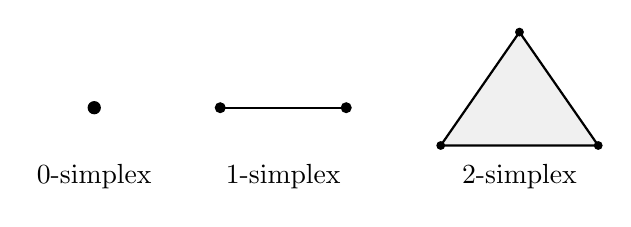
\begin{tikzpicture}[scale=0.8]
% 0-simplex
\fill (0,1) circle (3pt);
\node at (0,-0.1) {\(0\)-simplex};

% 1-simplex
\fill (2,1) circle (2.5pt);
\fill (4,1) circle (2.5pt);
\draw[thick] (2,1)--(4,1);
\node at (3,-0.1) {\(1\)-simplex};

% 2-simplex
\coordinate (A) at (5.5,0.4);
\coordinate (B) at (8,0.4);
\coordinate (C) at (6.75,2.2);
\filldraw[fill=gray!12,draw=black,thick] (A)--(B)--(C)--cycle;
\fill (A) circle (2pt);
\fill (B) circle (2pt);
\fill (C) circle (2pt);
\node at (6.75,-0.1) {\(2\)-simplex};
\end{tikzpicture}
\end{centereddiagram}

Higher-dimensional simplices generalize triangles and tetrahedra.

%%%%%%%%%%%%%%%%%%%%%%%%%%%%%%%%%%%%%%%%%%%%%%%%%%%%%%%%%%%%
\subsection{Barycentric Coordinates}
\label{subsec:barycentric-coordinates}
%%%%%%%%%%%%%%%%%%%%%%%%%%%%%%%%%%%%%%%%%%%%%%%%%%%%%%%%%%%%

Affine combinations provide a natural coordinate system relative to a
simplex.

\begin{definitionbox}{Barycentric Coordinates}
Let

\[ P_0,\ldots,P_k \]

be affinely independent.

Every point \(P\) in their affine hull can be written uniquely as

\[
\boxed{
P=\lambda_0P_0+\cdots+\lambda_kP_k,
\qquad
\lambda_0+\cdots+\lambda_k=1.
}
\]

The coefficients

\[ (\lambda_0,\ldots,\lambda_k) \]

are the \emph{barycentric coordinates} of \(P\) relative to the simplex.
\end{definitionbox}

The word \emph{barycentric} comes from the geometric idea of a center of
mass.

%%%%%%%%%%%%%%%%%%%%%%%%%%%%%%%%%%%%%%%%%%%%%%%%%%%%%%%%%%%%
\subsection{Barycentric Coordinates in a Triangle}
\label{subsec:barycentric-triangle}
%%%%%%%%%%%%%%%%%%%%%%%%%%%%%%%%%%%%%%%%%%%%%%%%%%%%%%%%%%%%

For a triangle with vertices \(A,B,C\),

\[
\boxed{
P=\lambda_AA+\lambda_BB+\lambda_CC,
\qquad
\lambda_A+\lambda_B+\lambda_C=1.
}
\]

If

\[
\lambda_A,\lambda_B,\lambda_C\geq0,
\]

then \(P\) lies inside or on the boundary of the triangle.

\begin{centereddiagram}
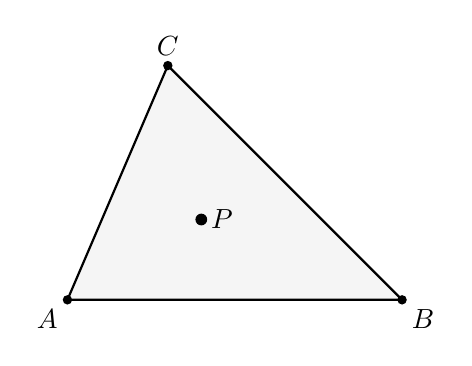
\begin{tikzpicture}[scale=0.85]
\coordinate (A) at (0,0);
\coordinate (B) at (5,0);
\coordinate (C) at (1.5,3.5);
\coordinate (P) at (2,1.2);

\filldraw[fill=gray!8,draw=black,thick] (A)--(B)--(C)--cycle;
\fill (A) circle (2pt);
\fill (B) circle (2pt);
\fill (C) circle (2pt);
\fill (P) circle (2.5pt);

\node[below left] at (A) {\(A\)};
\node[below right] at (B) {\(B\)};
\node[above] at (C) {\(C\)};
\node[right] at (P) {\(P\)};
\end{tikzpicture}
\end{centereddiagram}

%%%%%%%%%%%%%%%%%%%%%%%%%%%%%%%%%%%%%%%%%%%%%%%%%%%%%%%%%%%%
\subsection{Worked Example: Barycentric Coordinates}
\label{subsec:worked-barycentric-coordinates}
%%%%%%%%%%%%%%%%%%%%%%%%%%%%%%%%%%%%%%%%%%%%%%%%%%%%%%%%%%%%

\begin{workedexamplebox}{Barycentric Coordinates in a Triangle}

Let

\[
A=(0,0),\qquad
B=(4,0),\qquad
C=(0,4).
\]

Find barycentric coordinates of

\[ P=(1,1). \]

Write

\[ P=\lambda_AA+\lambda_BB+\lambda_CC. \]

\begin{tabularx}{\textwidth}{@{}>{\raggedright\arraybackslash}p{0.43\textwidth}X@{}}
Compare the \(x\)-coordinate. &
\(1=4\lambda_B\), so \(\lambda_B=\frac14\)\\
Compare the \(y\)-coordinate. &
\(1=4\lambda_C\), so \(\lambda_C=\frac14\)\\
Use the sum condition. &
\(\lambda_A+\frac14+\frac14=1\)\\
Solve. &
\(\lambda_A=\frac12\)
\end{tabularx}

\begin{answerbox}
\[ \boxed{(\lambda_A,\lambda_B,\lambda_C)=\left(\frac12,\frac14,\frac14\right)} \]
\end{answerbox}
\end{workedexamplebox}

%%%%%%%%%%%%%%%%%%%%%%%%%%%%%%%%%%%%%%%%%%%%%%%%%%%%%%%%%%%%
\subsection{Convex Combinations}
\label{subsec:affine-convex-combinations}
%%%%%%%%%%%%%%%%%%%%%%%%%%%%%%%%%%%%%%%%%%%%%%%%%%%%%%%%%%%%

An affine combination becomes a convex combination when all coefficients are
nonnegative.

\begin{definitionbox}{Convex Combination}
A \emph{convex combination} has the form

\[
\boxed{
\lambda_1P_1+\cdots+\lambda_kP_k
}
\]

where

\[
\boxed{
\lambda_i\geq0,
\qquad
\sum_{i=1}^{k}\lambda_i=1.
}
\]
\end{definitionbox}

Convex combinations describe points lying ``between'' other points in an
affine sense.

%%%%%%%%%%%%%%%%%%%%%%%%%%%%%%%%%%%%%%%%%%%%%%%%%%%%%%%%%%%%
\subsection{Convex Hull}
\label{subsec:convex-hull-affine}
%%%%%%%%%%%%%%%%%%%%%%%%%%%%%%%%%%%%%%%%%%%%%%%%%%%%%%%%%%%%

\begin{definitionbox}{Convex Hull}
The \emph{convex hull} of points \(P_1,\ldots,P_k\) is the set of all convex
combinations of those points:

\[
\boxed{
\operatorname{conv}\{P_1,\ldots,P_k\}
=
\left\{
\sum_{i=1}^{k}\lambda_iP_i:
\lambda_i\geq0,\ 
\sum_{i=1}^{k}\lambda_i=1
\right\}.
}
\]
\end{definitionbox}

The notation

\[ \operatorname{conv} \]

is read ``convex hull.''

For three noncollinear points, the convex hull is the filled triangle.

For four noncoplanar points in \(\R^3\), it is a tetrahedron.

Convexity is developed more fully in Convex Geometry and Convex
Optimization.

%%%%%%%%%%%%%%%%%%%%%%%%%%%%%%%%%%%%%%%%%%%%%%%%%%%%%%%%%%%%
\subsection{Centroids as Affine Combinations}
\label{subsec:centroids-affine}
%%%%%%%%%%%%%%%%%%%%%%%%%%%%%%%%%%%%%%%%%%%%%%%%%%%%%%%%%%%%

The centroid of points

\[ P_1,\ldots,P_k \]

is

\[
\boxed{
G=\frac1k(P_1+\cdots+P_k).
}
\]

Because

\[ \frac1k+\cdots+\frac1k=1, \]

the centroid is an affine combination.

For a triangle,

\[ \boxed{G=\frac13A+\frac13B+\frac13C.} \]

Affine transformations preserve centroids.

%%%%%%%%%%%%%%%%%%%%%%%%%%%%%%%%%%%%%%%%%%%%%%%%%%%%%%%%%%%%
\subsection{Affine Transformations}
\label{subsec:affine-transformations}
%%%%%%%%%%%%%%%%%%%%%%%%%%%%%%%%%%%%%%%%%%%%%%%%%%%%%%%%%%%%

The central transformations of affine geometry combine a linear
transformation with a translation.

\begin{definitionbox}{Affine Transformation}
An \emph{affine transformation} has the form

\[
\boxed{
T(\mathbf{x})=A\mathbf{x}+\mathbf{b},
}
\]

where \(A\) is a linear transformation and \(\mathbf{b}\) is a fixed vector.
\end{definitionbox}

If \(A\) is invertible, then \(T\) is an invertible affine transformation,
also called an \emph{affine automorphism} of the space.

%%%%%%%%%%%%%%%%%%%%%%%%%%%%%%%%%%%%%%%%%%%%%%%%%%%%%%%%%%%%
\subsection{Linear Transformations as Affine Transformations}
\label{subsec:linear-as-affine}
%%%%%%%%%%%%%%%%%%%%%%%%%%%%%%%%%%%%%%%%%%%%%%%%%%%%%%%%%%%%

If

\[ \mathbf{b}=\mathbf{0}, \]

then

\[ T(\mathbf{x})=A\mathbf{x}. \]

Thus every linear transformation is affine.

But not every affine transformation is linear.

For example,

\[ T(\mathbf{x})=\mathbf{x}+\mathbf{b} \]

with \(\mathbf{b}\neq\mathbf{0}\) is a translation.

It does not fix the origin and therefore is not a linear transformation.

%%%%%%%%%%%%%%%%%%%%%%%%%%%%%%%%%%%%%%%%%%%%%%%%%%%%%%%%%%%%
\subsection{Basic Affine Transformations}
\label{subsec:basic-affine-transformations}
%%%%%%%%%%%%%%%%%%%%%%%%%%%%%%%%%%%%%%%%%%%%%%%%%%%%%%%%%%%%

Common affine transformations include:

\begin{itemize}
    \item translations;
    \item rotations;
    \item reflections;
    \item scalings;
    \item nonuniform scalings;
    \item shears;
    \item compositions of these transformations.
\end{itemize}

Rotations and reflections are special because they preserve more Euclidean
structure than general affine transformations.

%%%%%%%%%%%%%%%%%%%%%%%%%%%%%%%%%%%%%%%%%%%%%%%%%%%%%%%%%%%%
\subsection{Translation}
\label{subsec:affine-translation}
%%%%%%%%%%%%%%%%%%%%%%%%%%%%%%%%%%%%%%%%%%%%%%%%%%%%%%%%%%%%

A translation by vector \(\mathbf{b}\) is

\[ \boxed{T(\mathbf{x})=\mathbf{x}+\mathbf{b}.} \]

Every point moves by the same displacement.

\begin{centereddiagram}
\begin{tikzpicture}[scale=0.75]
\draw[thick] (0,0)--(2,0)--(1,1.8)--cycle;
\draw[thick,dashed] (4,1)--(6,1)--(5,2.8)--cycle;

\draw[-{Latex[length=3mm]},thick] (1,0.8)--(4.5,1.8);
\node[above] at (2.7,1.4) {\(\mathbf{b}\)};
\end{tikzpicture}
\end{centereddiagram}

Translations preserve all Euclidean distances and angles, and therefore also
all affine properties.

%%%%%%%%%%%%%%%%%%%%%%%%%%%%%%%%%%%%%%%%%%%%%%%%%%%%%%%%%%%%
\subsection{Scaling}
\label{subsec:affine-scaling}
%%%%%%%%%%%%%%%%%%%%%%%%%%%%%%%%%%%%%%%%%%%%%%%%%%%%%%%%%%%%

A uniform scaling centered at the origin has the form

\[ T(\mathbf{x})=c\mathbf{x}. \]

If \(c\neq0\), this is an invertible affine transformation.

Uniform scaling preserves angles but generally changes distances.

Nonuniform scaling may change both lengths and angles.

For example,

\[
T(x,y)=(2x,y)
\]

stretches horizontally but not vertically.

A circle may therefore become an ellipse.

%%%%%%%%%%%%%%%%%%%%%%%%%%%%%%%%%%%%%%%%%%%%%%%%%%%%%%%%%%%%
\subsection{Shear Transformations}
\label{subsec:affine-shear}
%%%%%%%%%%%%%%%%%%%%%%%%%%%%%%%%%%%%%%%%%%%%%%%%%%%%%%%%%%%%

A \emph{shear} shifts one coordinate by an amount depending on another.

For example,

\[
\boxed{
T(x,y)=(x+ky,y)
}
\]

has matrix

\[
A=
\begin{pmatrix}
1&k\\
0&1
\end{pmatrix}.
\]

A square becomes a parallelogram.

\begin{centereddiagram}
\begin{tikzpicture}[scale=0.7]
\draw[thick] (0,0)--(2,0)--(2,2)--(0,2)--cycle;

\draw[-{Latex[length=3mm]},thick] (2.8,1)--(4,1);

\draw[thick] (5,0)--(7,0)--(8,2)--(6,2)--cycle;

\node at (1,-0.5) {before};
\node at (6.5,-0.5) {after shear};
\end{tikzpicture}
\end{centereddiagram}

Angles change, but parallel lines remain parallel.

%%%%%%%%%%%%%%%%%%%%%%%%%%%%%%%%%%%%%%%%%%%%%%%%%%%%%%%%%%%%
\subsection{Worked Example: Affine Transformation}
\label{subsec:worked-affine-transformation}
%%%%%%%%%%%%%%%%%%%%%%%%%%%%%%%%%%%%%%%%%%%%%%%%%%%%%%%%%%%%

\begin{workedexamplebox}{Applying an Affine Transformation}

Let

\[
T(\mathbf{x})
=
\begin{pmatrix}
2&1\\
0&1
\end{pmatrix}
\mathbf{x}
+
\begin{pmatrix}
3\\
-2
\end{pmatrix}.
\]

Find \(T(1,4)\).

\begin{tabularx}{\textwidth}{@{}>{\raggedright\arraybackslash}p{0.43\textwidth}X@{}}
Write the point as a column vector. &
\(\mathbf{x}=\begin{pmatrix}1\\4\end{pmatrix}\)\\
Apply the matrix. &
\(\begin{pmatrix}2&1\\0&1\end{pmatrix}
\begin{pmatrix}1\\4\end{pmatrix}
=
\begin{pmatrix}6\\4\end{pmatrix}\)\\
Add the translation. &
\(\begin{pmatrix}6\\4\end{pmatrix}
+
\begin{pmatrix}3\\-2\end{pmatrix}
=
\begin{pmatrix}9\\2\end{pmatrix}\)
\end{tabularx}

\begin{answerbox}
\[ \boxed{T(1,4)=(9,2)} \]
\end{answerbox}
\end{workedexamplebox}

%%%%%%%%%%%%%%%%%%%%%%%%%%%%%%%%%%%%%%%%%%%%%%%%%%%%%%%%%%%%
\subsection{Affine Transformations Preserve Affine Combinations}
\label{subsec:affine-transformations-combinations}
%%%%%%%%%%%%%%%%%%%%%%%%%%%%%%%%%%%%%%%%%%%%%%%%%%%%%%%%%%%%

Affine transformations interact naturally with affine combinations.

\begin{theorem}[Preservation of Affine Combinations]
Let

\[ T(\mathbf{x})=A\mathbf{x}+\mathbf{b}. \]

If

\[ \lambda_1+\cdots+\lambda_k=1, \]

then

\[
\boxed{
T\left(\sum_{i=1}^{k}\lambda_iP_i\right)
=
\sum_{i=1}^{k}\lambda_iT(P_i).
}
\]
\end{theorem}

\begin{proof}
Using the affine form,

\[
T\left(\sum_i\lambda_iP_i\right)
=
A\left(\sum_i\lambda_iP_i\right)+\mathbf{b}.
\]

By linearity,

\[
=
\sum_i\lambda_iAP_i+\mathbf{b}.
\]

Since \(\sum_i\lambda_i=1\),

\[
\mathbf{b}
=
\sum_i\lambda_i\mathbf{b}.
\]

Therefore

\[
T\left(\sum_i\lambda_iP_i\right)
=
\sum_i\lambda_i(AP_i+\mathbf{b})
=
\sum_i\lambda_iT(P_i).
\]

Hence affine combinations are preserved.
\end{proof}

%%%%%%%%%%%%%%%%%%%%%%%%%%%%%%%%%%%%%%%%%%%%%%%%%%%%%%%%%%%%
\subsection{Lines Map to Lines}
\label{subsec:affine-lines-map-lines}
%%%%%%%%%%%%%%%%%%%%%%%%%%%%%%%%%%%%%%%%%%%%%%%%%%%%%%%%%%%%

Let a line be

\[ P+t(Q-P). \]

Applying an affine transformation gives

\[
T(P+t(Q-P)).
\]

Because this is an affine combination,

\[
T(P+t(Q-P))
=
T(P)+t(T(Q)-T(P)).
\]

Thus an invertible affine transformation maps lines to lines.

Similarly:

\begin{itemize}
    \item planes map to planes;
    \item affine subspaces map to affine subspaces;
    \item collinear points remain collinear.
\end{itemize}

%%%%%%%%%%%%%%%%%%%%%%%%%%%%%%%%%%%%%%%%%%%%%%%%%%%%%%%%%%%%
\subsection{Parallelism Is Preserved}
\label{subsec:affine-parallelism}
%%%%%%%%%%%%%%%%%%%%%%%%%%%%%%%%%%%%%%%%%%%%%%%%%%%%%%%%%%%%

Suppose two lines have the same direction vector \(\mathbf{v}\):

\[
L_1=P+t\mathbf{v},
\qquad
L_2=Q+s\mathbf{v}.
\]

Under

\[ T(\mathbf{x})=A\mathbf{x}+\mathbf{b}, \]

their direction vectors become

\[ A\mathbf{v}. \]

Thus both transformed lines have the same direction.

For invertible \(A\), nonzero direction vectors remain nonzero.

Therefore parallel lines remain parallel.

%%%%%%%%%%%%%%%%%%%%%%%%%%%%%%%%%%%%%%%%%%%%%%%%%%%%%%%%%%%%
\subsection{Ratios Along a Line}
\label{subsec:affine-ratios-line}
%%%%%%%%%%%%%%%%%%%%%%%%%%%%%%%%%%%%%%%%%%%%%%%%%%%%%%%%%%%%

Suppose \(P,Q,R\) are collinear and

\[ R=(1-t)P+tQ. \]

The parameter \(t\) describes the relative position of \(R\) along the line.

Since affine transformations preserve affine combinations,

\[
T(R)
=
(1-t)T(P)+tT(Q).
\]

Thus the same parameter \(t\) describes the transformed point.

Consequently, affine transformations preserve ratios of directed segments
along a line.

In particular, they preserve:

\begin{itemize}
    \item midpoints;
    \item trisection points;
    \item centroids;
    \item general fixed affine ratios.
\end{itemize}

%%%%%%%%%%%%%%%%%%%%%%%%%%%%%%%%%%%%%%%%%%%%%%%%%%%%%%%%%%%%
\subsection{What Affine Transformations Preserve}
\label{subsec:affine-invariants}
%%%%%%%%%%%%%%%%%%%%%%%%%%%%%%%%%%%%%%%%%%%%%%%%%%%%%%%%%%%%

For invertible affine transformations:

\[
\begin{array}{c|c}
\textbf{Property} & \textbf{Preserved?}\\
\hline
points & \text{yes}\\
lines & \text{yes}\\
planes & \text{yes}\\
collinearity & \text{yes}\\
coplanarity & \text{yes}\\
parallelism & \text{yes}\\
affine dimension & \text{yes}\\
midpoints & \text{yes}\\
ratios along a line & \text{yes}\\
convex combinations & \text{yes}\\
length & \text{not generally}\\
angle & \text{not generally}\\
perpendicularity & \text{not generally}\\
circle shape & \text{not generally}\\
ordinary area & \text{not generally}
\end{array}
\]

This table summarizes the central distinction between affine and Euclidean
geometry.

%%%%%%%%%%%%%%%%%%%%%%%%%%%%%%%%%%%%%%%%%%%%%%%%%%%%%%%%%%%%
\subsection{Area and Volume Scaling}
\label{subsec:affine-area-volume-scaling}
%%%%%%%%%%%%%%%%%%%%%%%%%%%%%%%%%%%%%%%%%%%%%%%%%%%%%%%%%%%%

Although an affine transformation need not preserve area or volume, the
linear part determines how these quantities scale.

For

\[ T(\mathbf{x})=A\mathbf{x}+\mathbf{b}, \]

the translation \(\mathbf{b}\) does not affect area or volume.

In two dimensions,

\[
\boxed{
\text{area scale factor}=|\det A|.
}
\]

In three dimensions,

\[
\boxed{
\text{volume scale factor}=|\det A|.
}
\]

More generally, determinants measure oriented volume scaling in the
appropriate dimension.

%%%%%%%%%%%%%%%%%%%%%%%%%%%%%%%%%%%%%%%%%%%%%%%%%%%%%%%%%%%%
\subsection{Orientation Under Affine Transformations}
\label{subsec:affine-orientation}
%%%%%%%%%%%%%%%%%%%%%%%%%%%%%%%%%%%%%%%%%%%%%%%%%%%%%%%%%%%%

For an invertible affine transformation

\[ T(\mathbf{x})=A\mathbf{x}+\mathbf{b}, \]

the sign of \(\det A\) determines whether orientation is preserved.

\[
\begin{array}{c|c}
\det A & \textbf{Effect}\\
\hline
>0 & \text{orientation preserved}\\
<0 & \text{orientation reversed}
\end{array}
\]

If

\[ \det A=0, \]

the transformation is not invertible and collapses dimension.

%%%%%%%%%%%%%%%%%%%%%%%%%%%%%%%%%%%%%%%%%%%%%%%%%%%%%%%%%%%%
\subsection{Degenerate Affine Maps}
\label{subsec:degenerate-affine-maps}
%%%%%%%%%%%%%%%%%%%%%%%%%%%%%%%%%%%%%%%%%%%%%%%%%%%%%%%%%%%%

Not every affine map is invertible.

Consider

\[
T(x,y)=(x,0).
\]

This maps the entire plane onto the \(x\)-axis.

Its linear part is

\[
A=
\begin{pmatrix}
1&0\\
0&0
\end{pmatrix},
\]

and

\[ \det A=0. \]

Thus dimension can collapse under noninvertible affine maps.

When discussing affine equivalence and preservation of dimension, invertible
affine transformations are therefore essential.

%%%%%%%%%%%%%%%%%%%%%%%%%%%%%%%%%%%%%%%%%%%%%%%%%%%%%%%%%%%%
\subsection{Composition of Affine Transformations}
\label{subsec:composition-affine-transformations}
%%%%%%%%%%%%%%%%%%%%%%%%%%%%%%%%%%%%%%%%%%%%%%%%%%%%%%%%%%%%

Let

\[
T_1(\mathbf{x})=A_1\mathbf{x}+\mathbf{b}_1
\]

and

\[
T_2(\mathbf{x})=A_2\mathbf{x}+\mathbf{b}_2.
\]

Then

\[
T_2(T_1(\mathbf{x}))
=
A_2(A_1\mathbf{x}+\mathbf{b}_1)+\mathbf{b}_2.
\]

Therefore

\[
\boxed{
(T_2\circ T_1)(\mathbf{x})
=
(A_2A_1)\mathbf{x}
+
(A_2\mathbf{b}_1+\mathbf{b}_2).
}
\]

The composition of affine transformations is again affine.

%%%%%%%%%%%%%%%%%%%%%%%%%%%%%%%%%%%%%%%%%%%%%%%%%%%%%%%%%%%%
\subsection{Inverse Affine Transformations}
\label{subsec:inverse-affine-transformations}
%%%%%%%%%%%%%%%%%%%%%%%%%%%%%%%%%%%%%%%%%%%%%%%%%%%%%%%%%%%%

Suppose

\[ T(\mathbf{x})=A\mathbf{x}+\mathbf{b} \]

and \(A\) is invertible.

Set

\[ \mathbf{y}=A\mathbf{x}+\mathbf{b}. \]

Then

\[ \mathbf{y}-\mathbf{b}=A\mathbf{x}, \]

so

\[ \mathbf{x}=A^{-1}(\mathbf{y}-\mathbf{b}). \]

Therefore

\[
\boxed{
T^{-1}(\mathbf{y})
=
A^{-1}\mathbf{y}
-
A^{-1}\mathbf{b}.
}
\]

Thus the inverse of an invertible affine transformation is also affine.

%%%%%%%%%%%%%%%%%%%%%%%%%%%%%%%%%%%%%%%%%%%%%%%%%%%%%%%%%%%%
\subsection{The Affine Group}
\label{subsec:affine-group}
%%%%%%%%%%%%%%%%%%%%%%%%%%%%%%%%%%%%%%%%%%%%%%%%%%%%%%%%%%%%

The invertible affine transformations of \(\R^n\) form a group under
composition.

This group is called the \emph{affine group}.

It is commonly denoted

\[ \operatorname{Aff}(n,\R). \]

The notation is read ``the affine group of \(n\)-dimensional real affine
space.''

Every element has the form

\[ \mathbf{x}\mapsto A\mathbf{x}+\mathbf{b} \]

with

\[ A\in GL(n,\R),\qquad \mathbf{b}\in\R^n. \]

Here \(GL(n,\R)\) is the general linear group introduced in Group Theory and
Linear Algebra.

%%%%%%%%%%%%%%%%%%%%%%%%%%%%%%%%%%%%%%%%%%%%%%%%%%%%%%%%%%%%
\subsection{Homogeneous Coordinates}
\label{subsec:affine-homogeneous-coordinates}
%%%%%%%%%%%%%%%%%%%%%%%%%%%%%%%%%%%%%%%%%%%%%%%%%%%%%%%%%%%%

Translations are affine but not linear in ordinary \(n\)-dimensional
coordinates.

They can be incorporated into matrix multiplication by introducing one
additional coordinate.

A point

\[ \mathbf{x}=(x_1,\ldots,x_n) \]

is represented as

\[
\boxed{
\widetilde{\mathbf{x}}
=
\begin{pmatrix}
x_1\\
\vdots\\
x_n\\
1
\end{pmatrix}.
}
\]

The tilde in \(\widetilde{\mathbf{x}}\) is read ``x tilde.''

These are called \emph{homogeneous coordinates}.

%%%%%%%%%%%%%%%%%%%%%%%%%%%%%%%%%%%%%%%%%%%%%%%%%%%%%%%%%%%%
\subsection{Affine Transformations as Matrices}
\label{subsec:affine-homogeneous-matrix}
%%%%%%%%%%%%%%%%%%%%%%%%%%%%%%%%%%%%%%%%%%%%%%%%%%%%%%%%%%%%

The affine transformation

\[ T(\mathbf{x})=A\mathbf{x}+\mathbf{b} \]

can be represented by

\[
\boxed{
\begin{pmatrix}
A & \mathbf{b}\\
\mathbf{0}^{T} & 1
\end{pmatrix}.
}
\]

Thus

\[
\begin{pmatrix}
A & \mathbf{b}\\
\mathbf{0}^{T} & 1
\end{pmatrix}
\begin{pmatrix}
\mathbf{x}\\
1
\end{pmatrix}
=
\begin{pmatrix}
A\mathbf{x}+\mathbf{b}\\
1
\end{pmatrix}.
\]

Translation and linear transformation are now represented by one matrix
multiplication.

%%%%%%%%%%%%%%%%%%%%%%%%%%%%%%%%%%%%%%%%%%%%%%%%%%%%%%%%%%%%
\subsection{Two-Dimensional Homogeneous Coordinates}
\label{subsec:2d-homogeneous-coordinates}
%%%%%%%%%%%%%%%%%%%%%%%%%%%%%%%%%%%%%%%%%%%%%%%%%%%%%%%%%%%%

For

\[ T(x,y)=(ax+by+p,cx+dy+q), \]

the homogeneous matrix is

\[
\boxed{
\begin{pmatrix}
a&b&p\\
c&d&q\\
0&0&1
\end{pmatrix}.
}
\]

It acts on

\[
\begin{pmatrix}
x\\
y\\
1
\end{pmatrix}.
\]

This representation is standard in computer graphics, robotics, and
geometric computation.

%%%%%%%%%%%%%%%%%%%%%%%%%%%%%%%%%%%%%%%%%%%%%%%%%%%%%%%%%%%%
\subsection{Worked Example: Homogeneous Translation}
\label{subsec:worked-homogeneous-translation}
%%%%%%%%%%%%%%%%%%%%%%%%%%%%%%%%%%%%%%%%%%%%%%%%%%%%%%%%%%%%

\begin{workedexamplebox}{Translation Using Homogeneous Coordinates}

Translate the point

\[ P=(2,3) \]

by

\[ \mathbf{b}=(4,-1). \]

The homogeneous transformation matrix is

\[
T=
\begin{pmatrix}
1&0&4\\
0&1&-1\\
0&0&1
\end{pmatrix}.
\]

\begin{tabularx}{\textwidth}{@{}>{\raggedright\arraybackslash}p{0.43\textwidth}X@{}}
Write the point homogeneously. &
\(\widetilde{P}=\begin{pmatrix}2\\3\\1\end{pmatrix}\)\\
Multiply. &
\(\begin{pmatrix}1&0&4\\0&1&-1\\0&0&1\end{pmatrix}
\begin{pmatrix}2\\3\\1\end{pmatrix}
=
\begin{pmatrix}6\\2\\1\end{pmatrix}\)\\
Return to ordinary coordinates. &
\(T(P)=(6,2)\)
\end{tabularx}

\begin{answerbox}
\[ \boxed{T(P)=(6,2)} \]
\end{answerbox}
\end{workedexamplebox}

%%%%%%%%%%%%%%%%%%%%%%%%%%%%%%%%%%%%%%%%%%%%%%%%%%%%%%%%%%%%
\subsection{Parallel Lines and Points at Infinity}
\label{subsec:affine-parallel-projective-preview}
%%%%%%%%%%%%%%%%%%%%%%%%%%%%%%%%%%%%%%%%%%%%%%%%%%%%%%%%%%%%

Parallel lines are fundamentally different from intersecting lines in affine
geometry.

For example,

\[ y=0 \]

and

\[ y=1 \]

never meet in the affine plane.

Projective geometry extends affine geometry by introducing ideal points so
that parallel lines can be regarded as meeting at points at infinity.

This idea motivates the next section on Projective Geometry.

%%%%%%%%%%%%%%%%%%%%%%%%%%%%%%%%%%%%%%%%%%%%%%%%%%%%%%%%%%%%
\subsection{Affine Geometry and Coordinate Changes}
\label{subsec:affine-coordinate-changes}
%%%%%%%%%%%%%%%%%%%%%%%%%%%%%%%%%%%%%%%%%%%%%%%%%%%%%%%%%%%%

Changing an affine coordinate system involves choosing:

\begin{itemize}
    \item a new origin;
    \item a new basis of direction vectors.
\end{itemize}

If the old coordinates are \(\mathbf{x}\) and the new coordinates are
\(\mathbf{x}'\), the relationship has affine form

\[ \boxed{\mathbf{x}=A\mathbf{x}'+\mathbf{b}.} \]

Thus affine transformations naturally describe changes between coordinate
frames.

%%%%%%%%%%%%%%%%%%%%%%%%%%%%%%%%%%%%%%%%%%%%%%%%%%%%%%%%%%%%
\subsection{Affine Frames}
\label{subsec:affine-frames}
%%%%%%%%%%%%%%%%%%%%%%%%%%%%%%%%%%%%%%%%%%%%%%%%%%%%%%%%%%%%

An affine coordinate system can be specified by a point \(O\) and a basis

\[ \mathbf{e}_1,\ldots,\mathbf{e}_n \]

of the direction space.

Every point \(P\) can then be written uniquely as

\[
\boxed{
P=O+x_1\mathbf{e}_1+\cdots+x_n\mathbf{e}_n.
}
\]

The collection

\[ (O;\mathbf{e}_1,\ldots,\mathbf{e}_n) \]

is called an \emph{affine frame}.

Unlike a vector-space basis, an affine frame includes a chosen origin.

%%%%%%%%%%%%%%%%%%%%%%%%%%%%%%%%%%%%%%%%%%%%%%%%%%%%%%%%%%%%
\subsection{Affine Maps Determined by a Frame}
\label{subsec:affine-map-frame}
%%%%%%%%%%%%%%%%%%%%%%%%%%%%%%%%%%%%%%%%%%%%%%%%%%%%%%%%%%%%

An affine transformation in \(n\)-dimensional space is determined by its
action on \(n+1\) affinely independent points.

For example, an affine transformation of the plane is determined by where it
sends three noncollinear points.

An affine transformation of three-dimensional space is determined by where
it sends four noncoplanar points.

This follows because affine transformations preserve affine combinations.

%%%%%%%%%%%%%%%%%%%%%%%%%%%%%%%%%%%%%%%%%%%%%%%%%%%%%%%%%%%%
\subsection{Worked Example: Determining an Affine Map}
\label{subsec:worked-determine-affine-map}
%%%%%%%%%%%%%%%%%%%%%%%%%%%%%%%%%%%%%%%%%%%%%%%%%%%%%%%%%%%%

\begin{workedexamplebox}{Affine Map from Three Points}

Suppose an affine map \(T:\R^2\to\R^2\) satisfies

\[
T(0,0)=(1,1),\qquad
T(1,0)=(3,1),\qquad
T(0,1)=(2,4).
\]

Find \(T(x,y)\).

Write

\[ T(\mathbf{x})=A\mathbf{x}+\mathbf{b}. \]

\begin{tabularx}{\textwidth}{@{}>{\raggedright\arraybackslash}p{0.43\textwidth}X@{}}
Use \(T(0,0)\). &
\(\mathbf{b}=(1,1)\)\\
Use \(T(1,0)\). &
\(A(1,0)=(2,0)\)\\
Use \(T(0,1)\). &
\(A(0,1)=(1,3)\)\\
Construct \(A\). &
\(A=\begin{pmatrix}2&1\\0&3\end{pmatrix}\)
\end{tabularx}

Therefore

\[
T(x,y)
=
\begin{pmatrix}
2&1\\
0&3
\end{pmatrix}
\begin{pmatrix}
x\\
y
\end{pmatrix}
+
\begin{pmatrix}
1\\
1
\end{pmatrix}.
\]

\begin{answerbox}
\[ \boxed{T(x,y)=(2x+y+1,\,3y+1)} \]
\end{answerbox}
\end{workedexamplebox}

%%%%%%%%%%%%%%%%%%%%%%%%%%%%%%%%%%%%%%%%%%%%%%%%%%%%%%%%%%%%
\subsection{Affine Equivalence}
\label{subsec:affine-equivalence}
%%%%%%%%%%%%%%%%%%%%%%%%%%%%%%%%%%%%%%%%%%%%%%%%%%%%%%%%%%%%

Two geometric figures are \emph{affinely equivalent} if an invertible affine
transformation maps one onto the other.

For example:

\begin{itemize}
    \item every nondegenerate triangle is affinely equivalent to every other
    nondegenerate triangle;
    \item every parallelogram is affinely equivalent to a square;
    \item every nondegenerate ellipse is affinely equivalent to a circle.
\end{itemize}

Thus affine geometry classifies figures more coarsely than Euclidean
geometry.

%%%%%%%%%%%%%%%%%%%%%%%%%%%%%%%%%%%%%%%%%%%%%%%%%%%%%%%%%%%%
\subsection{Triangles Are Affinely Equivalent}
\label{subsec:triangles-affinely-equivalent}
%%%%%%%%%%%%%%%%%%%%%%%%%%%%%%%%%%%%%%%%%%%%%%%%%%%%%%%%%%%%

Let

\[ A,B,C \]

and

\[ A',B',C' \]

be two triples of noncollinear points.

Because each triple forms an affine frame for the plane, there exists a
unique affine transformation satisfying

\[
T(A)=A',\qquad
T(B)=B',\qquad
T(C)=C'.
\]

Consequently, any affine property proved for one convenient triangle can be
transferred to every nondegenerate triangle.

This is a powerful proof strategy.

%%%%%%%%%%%%%%%%%%%%%%%%%%%%%%%%%%%%%%%%%%%%%%%%%%%%%%%%%%%%
\subsection{Affine Proof Strategy}
\label{subsec:affine-proof-strategy}
%%%%%%%%%%%%%%%%%%%%%%%%%%%%%%%%%%%%%%%%%%%%%%%%%%%%%%%%%%%%

Suppose a geometric statement is invariant under affine transformations.

Instead of proving it for an arbitrary triangle, one may transform the
triangle into a convenient reference triangle such as

\[
(0,0),\qquad
(1,0),\qquad
(0,1).
\]

The theorem can then be proved using simple coordinates.

If every part of the statement is affine invariant, the result transfers
back to the original triangle.

\begin{warningbox}
This method cannot be used blindly for statements involving lengths, angles,
perpendicularity, or circles because these are not general affine
invariants.
\end{warningbox}

%%%%%%%%%%%%%%%%%%%%%%%%%%%%%%%%%%%%%%%%%%%%%%%%%%%%%%%%%%%%
\subsection{Ceva-Type Affine Structure}
\label{subsec:affine-ceva-structure}
%%%%%%%%%%%%%%%%%%%%%%%%%%%%%%%%%%%%%%%%%%%%%%%%%%%%%%%%%%%%

Many classical triangle theorems depend only on:

\begin{itemize}
    \item lines;
    \item intersections;
    \item ratios of points along sides.
\end{itemize}

Such statements often have affine interpretations.

For example, concurrency properties involving cevians and ratios along the
sides of a triangle survive invertible affine transformations.

This provides a bridge between classical Euclidean geometry and more
structural geometric reasoning.

%%%%%%%%%%%%%%%%%%%%%%%%%%%%%%%%%%%%%%%%%%%%%%%%%%%%%%%%%%%%
\subsection{Affine Geometry and Linear Equations}
\label{subsec:affine-linear-equations}
%%%%%%%%%%%%%%%%%%%%%%%%%%%%%%%%%%%%%%%%%%%%%%%%%%%%%%%%%%%%

Systems of linear equations naturally define affine subspaces.

A system

\[ A\mathbf{x}=\mathbf{b} \]

has solution set

\[ \mathbf{x}=\mathbf{x}_0+\mathbf{v}, \]

where \(\mathbf{x}_0\) is one particular solution and

\[ \mathbf{v}\in\ker A. \]

Thus, whenever the system is consistent,

\[
\boxed{
\{\mathbf{x}:A\mathbf{x}=\mathbf{b}\}
=
\mathbf{x}_0+\ker A.
}
\]

The solution set is therefore an affine translate of the null space.

%%%%%%%%%%%%%%%%%%%%%%%%%%%%%%%%%%%%%%%%%%%%%%%%%%%%%%%%%%%%
\subsection{Example: Solution Set as an Affine Space}
\label{subsec:solution-set-affine}
%%%%%%%%%%%%%%%%%%%%%%%%%%%%%%%%%%%%%%%%%%%%%%%%%%%%%%%%%%%%

Consider

\[ x+y+z=1. \]

A particular solution is

\[ (1,0,0). \]

The corresponding homogeneous equation is

\[ x+y+z=0. \]

Therefore the solution plane is

\[
\boxed{
(1,0,0)+
\{(x,y,z):x+y+z=0\}.
}
\]

The first set specifies location.

The second specifies direction.

%%%%%%%%%%%%%%%%%%%%%%%%%%%%%%%%%%%%%%%%%%%%%%%%%%%%%%%%%%%%
\subsection{Affine Geometry and Convex Geometry}
\label{subsec:affine-convex-geometry}
%%%%%%%%%%%%%%%%%%%%%%%%%%%%%%%%%%%%%%%%%%%%%%%%%%%%%%%%%%%%

Convex geometry is built naturally on affine geometry.

Convexity depends on line segments:

\[
(1-t)P+tQ,\qquad0\leq t\leq1.
\]

Because affine transformations preserve these combinations, they preserve
convexity.

If \(C\) is convex and \(T\) is affine, then

\[ T(C) \]

is convex.

This makes affine transformations central tools in convex analysis and
optimization.

%%%%%%%%%%%%%%%%%%%%%%%%%%%%%%%%%%%%%%%%%%%%%%%%%%%%%%%%%%%%
\subsection{Affine Geometry and Computational Geometry}
\label{subsec:affine-computational-geometry}
%%%%%%%%%%%%%%%%%%%%%%%%%%%%%%%%%%%%%%%%%%%%%%%%%%%%%%%%%%%%

Computational geometry frequently uses affine concepts such as:

\begin{itemize}
    \item orientation;
    \item convex hulls;
    \item barycentric coordinates;
    \item point-in-triangle tests;
    \item simplex representations;
    \item affine transformations;
    \item coordinate changes.
\end{itemize}

Barycentric coordinates are especially useful because they allow points to
be represented relative to triangle or tetrahedron vertices.

%%%%%%%%%%%%%%%%%%%%%%%%%%%%%%%%%%%%%%%%%%%%%%%%%%%%%%%%%%%%
\subsection{Affine Geometry and Computer Graphics}
\label{subsec:affine-computer-graphics}
%%%%%%%%%%%%%%%%%%%%%%%%%%%%%%%%%%%%%%%%%%%%%%%%%%%%%%%%%%%%

Computer graphics uses affine transformations to manipulate objects.

Typical operations include:

\[
\text{translate},
\quad
\text{rotate},
\quad
\text{scale},
\quad
\text{reflect},
\quad
\text{shear}.
\]

Using homogeneous coordinates, all of these can be represented by matrices.

Complex transformations can therefore be composed by matrix multiplication.

%%%%%%%%%%%%%%%%%%%%%%%%%%%%%%%%%%%%%%%%%%%%%%%%%%%%%%%%%%%%
\subsection{Affine Geometry and Robotics}
\label{subsec:affine-robotics}
%%%%%%%%%%%%%%%%%%%%%%%%%%%%%%%%%%%%%%%%%%%%%%%%%%%%%%%%%%%%

Robotic systems use coordinate frames to describe positions of:

\begin{itemize}
    \item joints;
    \item sensors;
    \item tools;
    \item objects;
    \item world coordinates.
\end{itemize}

Changing between frames requires transformations combining rotations and
translations.

These are special affine transformations.

Homogeneous transformation matrices allow these operations to be composed
efficiently.

%%%%%%%%%%%%%%%%%%%%%%%%%%%%%%%%%%%%%%%%%%%%%%%%%%%%%%%%%%%%
\subsection{Affine Geometry and Statistics}
\label{subsec:affine-statistics}
%%%%%%%%%%%%%%%%%%%%%%%%%%%%%%%%%%%%%%%%%%%%%%%%%%%%%%%%%%%%

Affine transformations also appear in statistics.

Data vectors may be transformed by

\[ \mathbf{y}=A\mathbf{x}+\mathbf{b}. \]

Translation changes the location of a data cloud, while \(A\) may rotate,
scale, or shear it.

Many multivariate statistical methods study quantities whose behavior under
affine transformations is important.

%%%%%%%%%%%%%%%%%%%%%%%%%%%%%%%%%%%%%%%%%%%%%%%%%%%%%%%%%%%%
\subsection{Affine Geometry and Projective Geometry}
\label{subsec:affine-projective-connection}
%%%%%%%%%%%%%%%%%%%%%%%%%%%%%%%%%%%%%%%%%%%%%%%%%%%%%%%%%%%%

Affine geometry preserves parallelism.

Projective geometry removes the special distinction between parallel and
intersecting lines by adding points at infinity.

Conceptually,

\[
\boxed{
\text{Euclidean Geometry}
\longrightarrow
\text{Affine Geometry}
\longrightarrow
\text{Projective Geometry}
}
\]

successively forgets geometric structure.

Euclidean geometry remembers distances and angles.

Affine geometry remembers parallelism but not general distance or angle.

Projective geometry remembers incidence but does not preserve affine
parallelism as a distinguished relation.

%%%%%%%%%%%%%%%%%%%%%%%%%%%%%%%%%%%%%%%%%%%%%%%%%%%%%%%%%%%%
\subsection{Hierarchy of Geometric Structure}
\label{subsec:geometric-structure-hierarchy}
%%%%%%%%%%%%%%%%%%%%%%%%%%%%%%%%%%%%%%%%%%%%%%%%%%%%%%%%%%%%

A useful structural picture is:

\begin{centereddiagram}
\begin{tikzpicture}[
node distance=9mm,
every node/.style={draw,rounded corners,minimum width=4.5cm,
minimum height=8mm,align=center}
]
\node (e) {Euclidean Geometry};
\node (a) [below=of e] {Affine Geometry};
\node (p) [below=of a] {Projective Geometry};

\draw[-{Latex[length=3mm]},thick] (e)--(a)
node[midway,right,draw=none,minimum width=0pt] {forget metric structure};

\draw[-{Latex[length=3mm]},thick] (a)--(p)
node[midway,right,draw=none,minimum width=0pt] {forget affine structure};
\end{tikzpicture}
\end{centereddiagram}

Each step retains fewer invariants and permits a larger class of
transformations.

%%%%%%%%%%%%%%%%%%%%%%%%%%%%%%%%%%%%%%%%%%%%%%%%%%%%%%%%%%%%
\subsection{Common Errors}
\label{subsec:affine-geometry-common-errors}
%%%%%%%%%%%%%%%%%%%%%%%%%%%%%%%%%%%%%%%%%%%%%%%%%%%%%%%%%%%%

\subsubsection{Treating Points as Ordinary Vectors}

Although coordinates allow points to be represented numerically by vectors,
affine geometry distinguishes locations from displacements.

The expression

\[ Q-P \]

has intrinsic meaning as a vector.

The expression

\[ P+Q \]

does not have intrinsic affine meaning without additional structure.

%%%%%%%%%%%%%%%%%%%%%%%%%%%%%%%%%%%%%%%%%%%%%%%%%%%%%%%%%%%%
\subsubsection{Forgetting the Sum-to-One Condition}

An affine combination requires

\[ \boxed{\sum_i\lambda_i=1.} \]

Without this condition, the expression generally depends on the chosen
origin.

%%%%%%%%%%%%%%%%%%%%%%%%%%%%%%%%%%%%%%%%%%%%%%%%%%%%%%%%%%%%
\subsubsection{Confusing Affine and Convex Combinations}

Affine combinations require only

\[ \sum_i\lambda_i=1. \]

Convex combinations additionally require

\[ \lambda_i\geq0. \]

Thus every convex combination is affine, but not every affine combination is
convex.

%%%%%%%%%%%%%%%%%%%%%%%%%%%%%%%%%%%%%%%%%%%%%%%%%%%%%%%%%%%%
\subsubsection{Confusing Affine and Linear Subspaces}

A linear subspace must contain the origin.

An affine subspace may be translated away from the origin.

For example,

\[ y=1 \]

is an affine line but not a linear subspace of \(\R^2\).

%%%%%%%%%%%%%%%%%%%%%%%%%%%%%%%%%%%%%%%%%%%%%%%%%%%%%%%%%%%%
\subsubsection{Testing Points Directly for Linear Independence}

Affine independence should be tested using difference vectors.

For

\[ P_0,P_1,\ldots,P_k, \]

test

\[ P_1-P_0,\ldots,P_k-P_0 \]

for linear independence.

%%%%%%%%%%%%%%%%%%%%%%%%%%%%%%%%%%%%%%%%%%%%%%%%%%%%%%%%%%%%
\subsubsection{Assuming Affine Maps Preserve Length}

General affine transformations may stretch different directions by different
amounts.

Therefore length is not an affine invariant.

%%%%%%%%%%%%%%%%%%%%%%%%%%%%%%%%%%%%%%%%%%%%%%%%%%%%%%%%%%%%
\subsubsection{Assuming Affine Maps Preserve Angles}

Shears and nonuniform scalings change angles.

Thus perpendicular lines need not remain perpendicular.

%%%%%%%%%%%%%%%%%%%%%%%%%%%%%%%%%%%%%%%%%%%%%%%%%%%%%%%%%%%%
\subsubsection{Assuming Every Affine Map Is Invertible}

An affine map

\[ T(\mathbf{x})=A\mathbf{x}+\mathbf{b} \]

is invertible only when \(A\) is invertible.

If

\[ \det A=0, \]

dimension may collapse.

%%%%%%%%%%%%%%%%%%%%%%%%%%%%%%%%%%%%%%%%%%%%%%%%%%%%%%%%%%%%
\subsubsection{Calling a Translation Linear}

A nontrivial translation

\[ T(\mathbf{x})=\mathbf{x}+\mathbf{b} \]

does not satisfy

\[ T(\mathbf{0})=\mathbf{0}. \]

Therefore it is affine but not linear.

%%%%%%%%%%%%%%%%%%%%%%%%%%%%%%%%%%%%%%%%%%%%%%%%%%%%%%%%%%%%
\subsection{Applications and Connections}
\label{subsec:affine-geometry-applications}
%%%%%%%%%%%%%%%%%%%%%%%%%%%%%%%%%%%%%%%%%%%%%%%%%%%%%%%%%%%%

\begin{applicationbox}
\textbf{Linear Algebra.}
Affine spaces are modeled on vector spaces, and affine subspaces are
translations of linear subspaces.

\medskip

\textbf{Euclidean Geometry.}
Affine geometry retains lines, parallelism, incidence, and ratios while
discarding general distance and angle information.

\medskip

\textbf{Projective Geometry.}
Projective geometry extends affine geometry by incorporating points at
infinity and treating parallel lines projectively.

\medskip

\textbf{Convex Geometry.}
Convex combinations, convex hulls, simplices, and barycentric coordinates are
naturally affine constructions.

\medskip

\textbf{Algebraic Geometry.}
Affine spaces such as \(\mathbb{A}^n\) provide fundamental settings for
studying polynomial equations. The algebraic-geometric meaning of
``affine'' is developed in its canonical section.

\medskip

\textbf{Optimization.}
Linear equality constraints define affine feasible sets, while convex
optimization combines affine structure with convexity.

\medskip

\textbf{Computer Graphics.}
Translation, scaling, rotation, reflection, and shear are implemented using
affine transformations and homogeneous matrices.

\medskip

\textbf{Robotics.}
Coordinate frames and spatial transformations combine linear transformations
with translations.

\medskip

\textbf{Computational Geometry.}
Affine independence, orientation, convex hulls, simplices, and barycentric
coordinates are basic computational tools.

\medskip

\textbf{Finite Element Methods.}
Barycentric and simplex coordinates are used to map standard reference
elements to physical computational elements.
\end{applicationbox}

%%%%%%%%%%%%%%%%%%%%%%%%%%%%%%%%%%%%%%%%%%%%%%%%%%%%%%%%%%%%
\subsection{Exercises}
\label{subsec:affine-geometry-exercises}
%%%%%%%%%%%%%%%%%%%%%%%%%%%%%%%%%%%%%%%%%%%%%%%%%%%%%%%%%%%%

\begin{exercise}[1]
Determine whether

\[ \frac13P+\frac23Q \]

is an affine combination of \(P\) and \(Q\).
\end{exercise}

\begin{exercise}[1]
Determine whether

\[ 2P-Q \]

is an affine combination of \(P\) and \(Q\).
\end{exercise}

\begin{exercise}[1]
Determine whether

\[ 2P+Q \]

is an affine combination.
\end{exercise}

\begin{exercise}[2]
Let

\[ P=(1,2),\qquad Q=(7,5). \]

Find

\[ \frac23P+\frac13Q. \]
\end{exercise}

\begin{exercise}[2]
Write the midpoint of \(P\) and \(Q\) as an affine combination.
\end{exercise}

\begin{exercise}[2]
Show that

\[ P+t(Q-P) \]

can be rewritten as

\[ (1-t)P+tQ. \]
\end{exercise}

\begin{exercise}[2]
Describe geometrically the set

\[ \{(1-t)P+tQ:0\leq t\leq1\}. \]
\end{exercise}

\begin{exercise}[2]
Describe geometrically

\[ P+\operatorname{span}\{\mathbf{v}\} \]

when \(\mathbf{v}\neq\mathbf{0}\).
\end{exercise}

\begin{exercise}[2]
Explain why

\[ y=3x+2 \]

is an affine subspace of \(\R^2\) but not a linear subspace.
\end{exercise}

\begin{exercise}[2]
Find the direction space of

\[ y=4x-7. \]
\end{exercise}

\begin{exercise}[2]
Find the affine hull of

\[ (0,0),\qquad(1,0). \]
\end{exercise}

\begin{exercise}[2]
Find the affine hull of

\[ (0,0),\qquad(1,0),\qquad(0,1). \]
\end{exercise}

\begin{exercise}[2]
Determine whether

\[
(0,0),\qquad
(1,2),\qquad
(2,4)
\]

are affinely independent.
\end{exercise}

\begin{exercise}[2]
Determine whether

\[
(0,0),\qquad
(1,0),\qquad
(0,1)
\]

are affinely independent.
\end{exercise}

\begin{exercise}[3]
Determine the affine dimension of

\[
(1,1,1),\qquad
(2,1,1),\qquad
(1,2,1),\qquad
(3,4,1).
\]
\end{exercise}

\begin{exercise}[2]
Find the centroid of the triangle with vertices

\[ (0,0),\qquad(6,0),\qquad(0,9). \]
\end{exercise}

\begin{exercise}[3]
Find the barycentric coordinates of

\[ P=(2,1) \]

relative to

\[
A=(0,0),\qquad
B=(4,0),\qquad
C=(0,2).
\]
\end{exercise}

\begin{exercise}[2]
Determine whether

\[
\frac12P+\frac14Q+\frac14R
\]

is a convex combination.
\end{exercise}

\begin{exercise}[2]
Determine whether

\[
2P-Q
\]

is a convex combination.
\end{exercise}

\begin{exercise}[2]
Describe the convex hull of three noncollinear points in the plane.
\end{exercise}

\begin{exercise}[1]
Determine whether

\[ T(x,y)=(x+3,y-2) \]

is linear, affine, or both.
\end{exercise}

\begin{exercise}[1]
Determine whether

\[ T(x,y)=(2x,3y) \]

is linear, affine, or both.
\end{exercise}

\begin{exercise}[2]
Write

\[ T(x,y)=(2x+y+4,x-y-3) \]

in the form

\[ T(\mathbf{x})=A\mathbf{x}+\mathbf{b}. \]
\end{exercise}

\begin{exercise}[2]
Find the image of

\[ (2,-1) \]

under

\[ T(x,y)=(3x+y+2,x+2y-4). \]
\end{exercise}

\begin{exercise}[2]
Find the matrix of the shear

\[ T(x,y)=(x+2y,y). \]
\end{exercise}

\begin{exercise}[2]
Find the determinant of the linear part of

\[ T(x,y)=(3x+y,2y). \]

What is the corresponding area scale factor?
\end{exercise}

\begin{exercise}[2]
Determine whether the affine transformation

\[
T(\mathbf{x})
=
\begin{pmatrix}
1&2\\
2&4
\end{pmatrix}\mathbf{x}
+
\begin{pmatrix}
1\\
0
\end{pmatrix}
\]

is invertible.
\end{exercise}

\begin{exercise}[3]
Find the inverse of

\[ T(x,y)=(2x+1,3y-4). \]
\end{exercise}

\begin{exercise}[3]
Let

\[ T_1(\mathbf{x})=A_1\mathbf{x}+\mathbf{b}_1 \]

and

\[ T_2(\mathbf{x})=A_2\mathbf{x}+\mathbf{b}_2. \]

Derive the affine form of \(T_2\circ T_1\).
\end{exercise}

\begin{exercise}[2]
Write the homogeneous-coordinate matrix for translation by

\[ (5,-3). \]
\end{exercise}

\begin{exercise}[2]
Write the homogeneous-coordinate matrix for

\[ T(x,y)=(2x,3y). \]
\end{exercise}

\begin{exercise}[3]
Write a single homogeneous matrix that first scales by

\[ (x,y)\mapsto(2x,2y) \]

and then translates by

\[ (3,-1). \]
\end{exercise}

\begin{exercise}[3]
Prove that affine transformations preserve midpoints.
\end{exercise}

\begin{exercise}[3]
Prove that affine transformations preserve affine combinations.
\end{exercise}

\begin{exercise}[3]
Prove that an invertible affine transformation maps parallel lines to
parallel lines.
\end{exercise}

\begin{exercise}[3]
Show that an affine transformation maps convex combinations to convex
combinations.
\end{exercise}

\begin{exercise}[3]
Show that the solution set of a consistent system

\[ A\mathbf{x}=\mathbf{b} \]

is a translate of \(\ker A\).
\end{exercise}

\begin{exercise}[3]
Explain why every nondegenerate triangle is affinely equivalent to the
triangle with vertices

\[ (0,0),\qquad(1,0),\qquad(0,1). \]
\end{exercise}

\begin{exercise}[3]
Give an example of an affine transformation that does not preserve angles.
\end{exercise}

\begin{exercise}[3]
Give an example of an affine transformation that sends a circle to a
noncircular ellipse.
\end{exercise}

\begin{exercise}[3]
Explain why a theorem involving only collinearity, parallelism, and ratios
along lines is a natural candidate for an affine proof.
\end{exercise}

%%%%%%%%%%%%%%%%%%%%%%%%%%%%%%%%%%%%%%%%%%%%%%%%%%%%%%%%%%%%
\subsection{Conceptual Summary}
\label{subsec:affine-geometry-summary}
%%%%%%%%%%%%%%%%%%%%%%%%%%%%%%%%%%%%%%%%%%%%%%%%%%%%%%%%%%%%

Affine geometry studies geometric structure without requiring a preferred
origin or Euclidean metric.

An affine space distinguishes points from displacement vectors.

The difference of two points is a vector:

\[ \boxed{Q-P\in V.} \]

A vector can translate a point:

\[ \boxed{P+\mathbf{v}\in A.} \]

An affine combination satisfies

\[
\boxed{
\lambda_1P_1+\cdots+\lambda_kP_k,
\qquad
\sum_{i=1}^{k}\lambda_i=1.
}
\]

The affine hull is

\[
\boxed{
\operatorname{aff}\{P_1,\ldots,P_k\}
=
P_1+
\operatorname{span}\{P_2-P_1,\ldots,P_k-P_1\}.
}
\]

Points are affinely independent when their difference vectors are linearly
independent.

An affine subspace has the form

\[ \boxed{P+W.} \]

A convex combination additionally satisfies

\[ \boxed{\lambda_i\geq0.} \]

An affine transformation has the form

\[ \boxed{T(\mathbf{x})=A\mathbf{x}+\mathbf{b}.} \]

Invertible affine transformations preserve:

\[
\boxed{
\text{incidence},
\quad
\text{collinearity},
\quad
\text{parallelism},
\quad
\text{affine combinations},
\quad
\text{ratios along lines}.
}
\]

They do not generally preserve:

\[
\boxed{
\text{length},
\quad
\text{angle},
\quad
\text{perpendicularity}.
}
\]

Homogeneous coordinates allow affine transformations to be represented by
matrices:

\[
\boxed{
\begin{pmatrix}
A&\mathbf{b}\\
\mathbf{0}^{T}&1
\end{pmatrix}.
}
\]

Affine geometry therefore provides a structural language connecting vector
spaces, classical geometry, convexity, computational geometry, and
projective geometry.

%%%%%%%%%%%%%%%%%%%%%%%%%%%%%%%%%%%%%%%%%%%%%%%%%%%%%%%%%%%%
\subsection{Section Connections}
\label{subsec:affine-geometry-connections}
%%%%%%%%%%%%%%%%%%%%%%%%%%%%%%%%%%%%%%%%%%%%%%%%%%%%%%%%%%%%

\chapterconnection{
Affine Geometry builds directly on Vector Geometry from
\cref{sec:vector-geometry} but removes the requirement that the geometry
possess a distinguished origin, distance, or angle. Points form an affine
space whose differences are vectors, while affine combinations describe
lines, planes, simplices, centroids, and barycentric coordinates. Linear
Algebra supplies the direction spaces and linear parts of affine
transformations. Convex Geometry later develops convex combinations and
convex hulls systematically. Algebraic Geometry uses affine spaces as
fundamental settings for polynomial equations. The next section, Projective
Geometry, extends the affine viewpoint by adding points at infinity and
removing the special status of parallel lines.
}

%%%%%%%%%%%%%%%%%%%%%%%%%%%%%%%%%%%%%%%%%%%%%%%%%%%%%%%%%%%%
% SECTION SOURCE TRACKING
%%%%%%%%%%%%%%%%%%%%%%%%%%%%%%%%%%%%%%%%%%%%%%%%%%%%%%%%%%%%

%------------------------------------------------------------
% 3.4 Affine Geometry
%------------------------------------------------------------
%
% Source basis:
%   - Standard affine geometry and linear algebra.
%
% Used for:
%   - affine spaces and the point-vector distinction;
%   - affine combinations;
%   - affine lines and subspaces;
%   - affine hulls and affine independence;
%   - affine dimension;
%   - simplices and barycentric coordinates;
%   - convex combinations and convex hulls;
%   - affine transformations;
%   - translations, scalings, and shears;
%   - affine invariants;
%   - area and volume scaling;
%   - homogeneous coordinates;
%   - affine frames;
%   - solution sets of linear systems as affine spaces;
%   - connections with convex and projective geometry.
%
% Notes:
%   - Linear independence, span, rank, determinants, kernels,
%     and matrix transformations are canonical in Linear Algebra.
%   - Vector operations are canonical in Vector Geometry.
%   - Convexity is developed systematically in Convex Geometry.
%   - Projective completion and points at infinity belong
%     canonically to Projective Geometry.
%   - Algebraic affine spaces belong canonically to Algebraic
%     Geometry.
%
%%%%%%%%%%%%%%%%%%%%%%%%%%%%%%%%%%%%%%%%%%%%%%%%%%%%%%%%%%%%